\documentclass[a4paper,twoside,openright,makeidx,12pt]{book}
%\usepackage{draftcopy}
%%$Id: macro.tex,v 1.10 2004/12/08 13:38:58 acary Exp $


%\usepackage{a4wide}
\textheight 25cm
\textwidth 16.5cm
\topmargin -1cm
%\evensidemargin 0cm
\oddsidemargin 0cm
\evensidemargin0cm
\usepackage{layout}


\usepackage{amsmath}
\usepackage{amssymb}
\usepackage{minitoc}
%\usepackage{glosstex}
\usepackage{colortbl}
\usepackage{hhline}
\usepackage{longtable}

%\usepackage{glosstex}
%\def\glossaryname{Glossary of Notation}
\def\listacronymname{Acronyms}

\usepackage[outerbars]{changebar}\setcounter{changebargrey}{20}
%\glxitemorderdefault{acr}{l}

%\usepackage{color}
\usepackage{graphicx,epsfig}
\graphicspath{{./Figures/}}
\usepackage[T1]{fontenc}
\usepackage{rotating}

%\usepackage{algorithmic}
%\usepackage{algorithm}
\usepackage{ntheorem}
\usepackage{natbib}


%\renewcommand{\baselinestretch}{2.0}
\setcounter{tocdepth}{2}     % Dans la table des matieres
\setcounter{secnumdepth}{3}  % Avec un numero.



\newtheorem{definition}{Definition}
\newtheorem{lemma}{Lemma}
\newtheorem{claim}{Claim}
\newtheorem{remark}{Remark}
\newtheorem{assumption}{Assumption}
\newtheorem{example}{Example}
\newtheorem{conjecture}{Conjecture}
\newtheorem{corollary}{Corollary}
\newtheorem{OP}{OP}
\newtheorem{problem}{Problem}
\newtheorem{theorem}{Theorem}


\newcommand{\CC}{\mbox{\rm $~\vrule height6.6pt width0.5pt depth0.25pt\!\!$C}}
\newcommand{\ZZ}{\mbox{\rm \lower0.3pt\hbox{$\angle\!\!\!$}Z}}
\newcommand{\RR}{\mbox{\rm $I\!\!R$}}
\newcommand{\HH}{\mbox{\rm $I\!\!H$}}
\newcommand{\NN}{\mbox{\rm $I\!\!N$}}

\newcommand{\Mnn}{\mathcal M^{n\times n}}
\newcommand{\Mnp}[2]{\ensuremath{\mathcal M^{#1\times #2}}}



\newcommand{\Frac}[2]{\displaystyle \frac{#1}{#2}}

\newcommand{\DP}[2]{\displaystyle \frac{\partial {#1}}{\partial {#2}}}

% c++ variables writting
\newcommand{\varcpp}[1]{\textit{#1}}
% itemize
\newcommand{\bei}{\begin{itemize}}
\newcommand{\ei}{\end{itemize}}

\newcommand{\ie}{i.e.}
\newcommand{\eg}{e.g.}
\newcommand{\cf}{c.f.}
\newcommand{\putidx}[1]{\index{#1}\textit{#1}}

\def\Er{{\rm I\! R}}
\def\En{{\rm I\! N}} 
\def\Ec{{\rm I\! C}}
 
\def\zc{\hat{z}}
\def\wc{\hat{w}}

\font\tete=cmr8 at 8 pt


% normal tangent
\def\n{{\hbox{\tiny{N}}}}
\def\t{{\hbox{\tiny{T}}}}
\def\nt{\hbox{\tiny{NT}}}
\def\nsf{\hbox{\tiny{\textsf N}}}
\def\tsf{\hbox{\tiny{\textsf T}}}
\def\sigman{\sigma_{\n}}
\def\sigmat{\sigma_{\t}}
\def\sigmant{\sigma_{\nt}}
\def\epsn{\epsilon_{\n}}
\def\epst{\epsilon_{\t}}
\def\epsnt{\epsilon_{\nt}}
\def\eps{\epsilon}
\def\veps{\varepsilon}
\def\sig{\sigma}
\def\Rn{R_{\n}}
\def\Rt{R_{\t}}
\def\cn{c_{\n}}
\def\Cn{C_{\n}}
\def\ct{c_{\t}}
\def\Ct{C_{\t}}
\def\un{u_{\n}}
\def\ut{\buu_{\t}}
\def\uut{u_{\t}}
\def\unc{u_{\n}^c}
\def\utc{\buu_{\t}^c}
\def\vn{v_{\n}}
\def\vt{v_{\t}}
\def\rr{\hbox{\tiny{\textsf R}}}
\def\irr{\hbox{\tiny{\textsf{IR}}}}
\def\rn{r_{\n}}
\def\rt{\brr_{\t}}
\def\rnc{r_{\n}^c}
\def\rtc{\brr_{\t}^c}
\def\trn{\Tilde{r}_{\n}}
\def\trt{\Tilde{\brr}_{\t}}
\def\tr{\Tilde{\brr}}
\def\tv{\Tilde{\bvv}}
\def\vn{v_{\n}}
\def\vt{\bvv_{\t}}
\def\adh{\mathsf{adh}}
\def\adj{\hbox{\tiny{\textsf{adj}}}}
\def\adjc{\hbox{\tiny{\textsf{adjC}}}}
\def\adja{\hbox{\tiny{\textsf{adjA}}}}
\def\cc{\hbox{\tiny{\textsf C}}}
\def\ca{\hbox{\tiny{\textsf A}}}

\DeclareMathOperator{\proj}{proj}
\DeclareMathOperator{\expm}{expm}
\DeclareMathOperator{\dexp}{dexp}
\DeclareMathOperator{\dlexp}{d^l exp}
\DeclareMathOperator{\drexp}{d^r exp}
\DeclareMathOperator{\dexpm}{dexpm}
\DeclareMathOperator{\expq}{expq}
\DeclareMathOperator{\dexpq}{dexpq}
\DeclareMathOperator{\Ad}{Ad}
\DeclareMathOperator{\ad}{ad}
\DeclareMathOperator{\dd}{d}



%%  Les ensembles de nombres  C. Fiorio (fiorioÊatÊmath.tu-berlin.de) 
%
\def\nbR{\ensuremath{\mathrm{I\!R}}} % IR
\def\nbN{\ensuremath{\mathrm{I\!N}}} % IN
\def\nbF{\ensuremath{\mathrm{I\!F}}} % IF
\def\nbH{\ensuremath{\mathrm{I\!H}}} % IH
\def\nbK{\ensuremath{\mathrm{I\!K}}} % IK
\def\nbL{\ensuremath{\mathrm{I\!L}}} % IL
\def\nbM{\ensuremath{\mathrm{I\!M}}} % IM
\def\nbP{\ensuremath{\mathrm{I\!P}}} % IP

%----------------------------------------------------------------------
%                  Modification des subsubsections
%----------------------------------------------------------------------
\makeatletter
\renewcommand\thesubsubsection{\thesubsection.\@alph\c@subsubsection}
\makeatother

%----------------------------------------------------------------------
%             Redaction note environnement
%----------------------------------------------------------------------
\makeatletter
\theoremheaderfont{\scshape}
\theoremstyle{marginbreak}
\theorembodyfont{\upshape}
%\newtheorem{rque}{\bf Remarque}[chapter]
%\newtheorem{rque1}{\bf \fsc{Remarque}}[chapter] !!! \fsc est une commande french
\newtheorem{ndr1}{\textbf{\textsc{Redaction note}}}[section]

\newenvironment{ndr}%
{%
\tt
%\centerline{---oOo---}
\noindent\begin{ndr1}%
}%
{%
\begin{flushright}%
%\vspace{-1.5em}\ding{111}
\end{flushright}%
\end{ndr1}%
%\centerline{---oOo---}
}

\makeatother

%----------------------------------------------------------------------
%             Redaction note environnement V.ACARY
%----------------------------------------------------------------------
\makeatletter
\theoremheaderfont{\scshape}
\theoremstyle{marginbreak}
\theorembodyfont{\upshape}
%\newtheorem{rque}{\bf Remarque}[chapter]
%\newtheorem{rque1}{\bf \fsc{Remarque}}[chapter] !!! \fsc est une commande french
\newtheorem{ndr1va}{\textbf{\textsc{Redaction note V. ACARY}}}[section]

\newenvironment{ndrva}%
{%
\tt
%\centerline{---oOo---}
\noindent\begin{ndr1va}%
}%
{%
\begin{flushright}%
%\vspace{-1.5em}\ding{111}
\end{flushright}%
\end{ndr1va}%
%\centerline{---oOo---}
}

\makeatother
%----------------------------------------------------------------------
%             Redaction note environnement V.ACARY
%----------------------------------------------------------------------
\makeatletter
\theoremheaderfont{\scshape}
\theoremstyle{marginbreak}
\theorembodyfont{\upshape}
%\newtheorem{rque}{\bf Remarque}[chapter]
%\newtheorem{rque1}{\bf \fsc{Remarque}}[chapter] !!! \fsc est une commande french
\newtheorem{ndr1fp}{\textbf{\textsc{Redaction note F. PERIGNON}}}[section]

\newenvironment{ndrfp}%
{%
\tt
%\centerline{---oOo---}
\noindent\begin{ndr1fp}%
}%
{%
\begin{flushright}%
%\vspace{-1.5em}\ding{111}
\end{flushright}%
\end{ndr1fp}%
%\centerline{---oOo---}
}

\makeatother
%----------------------------------------------------------------------
%                  Chapter head enviroment
%----------------------------------------------------------------------
\newenvironment{chapter_head}
{%
\begin{center}%
-------------------- oOo --------------------\\%
\ \\%
\begin{minipage}[]{14cm}%
\noindent\normalsize\advance\baselineskip-1pt %
}%
{%
\par\end{minipage}%
\ \\%
\ \\%
-------------------- oOo --------------------
\end{center}%
\vspace*{\stretch{1}}%
\clearpage%
\thispagestyle{empty}%
\vspace*{\stretch{1}}%
\minitoc%
\vspace*{\stretch{2}}%
\clearpage%
}


\newcommand{\contract}{{\,:\,}}

%%% Local Variables: 
%%% mode: latex
%%% TeX-master: "report"
%%% End: 

%$Id: macro.tex,v 1.10 2004/12/08 13:38:58 acary Exp $


%\usepackage{a4wide}
\textheight 25cm
\textwidth 16.5cm
\topmargin -1cm
%\evensidemargin 0cm
\oddsidemargin 0cm
\evensidemargin0cm
\usepackage{layout}


\usepackage{amsmath}
\usepackage{amssymb}
\usepackage{minitoc}
%\usepackage{glosstex}
\usepackage{colortbl}
\usepackage{hhline}
\usepackage{longtable}

%\usepackage{glosstex}
%\def\glossaryname{Glossary of Notation}
\def\listacronymname{Acronyms}

\usepackage[outerbars]{changebar}\setcounter{changebargrey}{20}
%\glxitemorderdefault{acr}{l}

%\usepackage{color}
\usepackage{graphicx,epsfig}
\graphicspath{{./Figures/}}
\usepackage[T1]{fontenc}
\usepackage{rotating}

%\usepackage{algorithmic}
%\usepackage{algorithm}
\usepackage{ntheorem}
\usepackage{natbib}


%\renewcommand{\baselinestretch}{2.0}
\setcounter{tocdepth}{2}     % Dans la table des matieres
\setcounter{secnumdepth}{3}  % Avec un numero.



\newtheorem{definition}{Definition}
\newtheorem{lemma}{Lemma}
\newtheorem{claim}{Claim}
\newtheorem{remark}{Remark}
\newtheorem{assumption}{Assumption}
\newtheorem{example}{Example}
\newtheorem{conjecture}{Conjecture}
\newtheorem{corollary}{Corollary}
\newtheorem{OP}{OP}
\newtheorem{problem}{Problem}
\newtheorem{theorem}{Theorem}


\newcommand{\CC}{\mbox{\rm $~\vrule height6.6pt width0.5pt depth0.25pt\!\!$C}}
\newcommand{\ZZ}{\mbox{\rm \lower0.3pt\hbox{$\angle\!\!\!$}Z}}
\newcommand{\RR}{\mbox{\rm $I\!\!R$}}
\newcommand{\HH}{\mbox{\rm $I\!\!H$}}
\newcommand{\NN}{\mbox{\rm $I\!\!N$}}

\newcommand{\Mnn}{\mathcal M^{n\times n}}
\newcommand{\Mnp}[2]{\ensuremath{\mathcal M^{#1\times #2}}}



\newcommand{\Frac}[2]{\displaystyle \frac{#1}{#2}}

\newcommand{\DP}[2]{\displaystyle \frac{\partial {#1}}{\partial {#2}}}

% c++ variables writting
\newcommand{\varcpp}[1]{\textit{#1}}
% itemize
\newcommand{\bei}{\begin{itemize}}
\newcommand{\ei}{\end{itemize}}

\newcommand{\ie}{i.e.}
\newcommand{\eg}{e.g.}
\newcommand{\cf}{c.f.}
\newcommand{\putidx}[1]{\index{#1}\textit{#1}}

\def\Er{{\rm I\! R}}
\def\En{{\rm I\! N}} 
\def\Ec{{\rm I\! C}}
 
\def\zc{\hat{z}}
\def\wc{\hat{w}}

\font\tete=cmr8 at 8 pt


% normal tangent
\def\n{{\hbox{\tiny{N}}}}
\def\t{{\hbox{\tiny{T}}}}
\def\nt{\hbox{\tiny{NT}}}
\def\nsf{\hbox{\tiny{\textsf N}}}
\def\tsf{\hbox{\tiny{\textsf T}}}
\def\sigman{\sigma_{\n}}
\def\sigmat{\sigma_{\t}}
\def\sigmant{\sigma_{\nt}}
\def\epsn{\epsilon_{\n}}
\def\epst{\epsilon_{\t}}
\def\epsnt{\epsilon_{\nt}}
\def\eps{\epsilon}
\def\veps{\varepsilon}
\def\sig{\sigma}
\def\Rn{R_{\n}}
\def\Rt{R_{\t}}
\def\cn{c_{\n}}
\def\Cn{C_{\n}}
\def\ct{c_{\t}}
\def\Ct{C_{\t}}
\def\un{u_{\n}}
\def\ut{\buu_{\t}}
\def\uut{u_{\t}}
\def\unc{u_{\n}^c}
\def\utc{\buu_{\t}^c}
\def\vn{v_{\n}}
\def\vt{v_{\t}}
\def\rr{\hbox{\tiny{\textsf R}}}
\def\irr{\hbox{\tiny{\textsf{IR}}}}
\def\rn{r_{\n}}
\def\rt{\brr_{\t}}
\def\rnc{r_{\n}^c}
\def\rtc{\brr_{\t}^c}
\def\trn{\Tilde{r}_{\n}}
\def\trt{\Tilde{\brr}_{\t}}
\def\tr{\Tilde{\brr}}
\def\tv{\Tilde{\bvv}}
\def\vn{v_{\n}}
\def\vt{\bvv_{\t}}
\def\adh{\mathsf{adh}}
\def\adj{\hbox{\tiny{\textsf{adj}}}}
\def\adjc{\hbox{\tiny{\textsf{adjC}}}}
\def\adja{\hbox{\tiny{\textsf{adjA}}}}
\def\cc{\hbox{\tiny{\textsf C}}}
\def\ca{\hbox{\tiny{\textsf A}}}

\DeclareMathOperator{\proj}{proj}
\DeclareMathOperator{\expm}{expm}
\DeclareMathOperator{\dexp}{dexp}
\DeclareMathOperator{\dlexp}{d^l exp}
\DeclareMathOperator{\drexp}{d^r exp}
\DeclareMathOperator{\dexpm}{dexpm}
\DeclareMathOperator{\expq}{expq}
\DeclareMathOperator{\dexpq}{dexpq}
\DeclareMathOperator{\Ad}{Ad}
\DeclareMathOperator{\ad}{ad}
\DeclareMathOperator{\dd}{d}



%%  Les ensembles de nombres  C. Fiorio (fiorioÊatÊmath.tu-berlin.de) 
%
\def\nbR{\ensuremath{\mathrm{I\!R}}} % IR
\def\nbN{\ensuremath{\mathrm{I\!N}}} % IN
\def\nbF{\ensuremath{\mathrm{I\!F}}} % IF
\def\nbH{\ensuremath{\mathrm{I\!H}}} % IH
\def\nbK{\ensuremath{\mathrm{I\!K}}} % IK
\def\nbL{\ensuremath{\mathrm{I\!L}}} % IL
\def\nbM{\ensuremath{\mathrm{I\!M}}} % IM
\def\nbP{\ensuremath{\mathrm{I\!P}}} % IP

%----------------------------------------------------------------------
%                  Modification des subsubsections
%----------------------------------------------------------------------
\makeatletter
\renewcommand\thesubsubsection{\thesubsection.\@alph\c@subsubsection}
\makeatother

%----------------------------------------------------------------------
%             Redaction note environnement
%----------------------------------------------------------------------
\makeatletter
\theoremheaderfont{\scshape}
\theoremstyle{marginbreak}
\theorembodyfont{\upshape}
%\newtheorem{rque}{\bf Remarque}[chapter]
%\newtheorem{rque1}{\bf \fsc{Remarque}}[chapter] !!! \fsc est une commande french
\newtheorem{ndr1}{\textbf{\textsc{Redaction note}}}[section]

\newenvironment{ndr}%
{%
\tt
%\centerline{---oOo---}
\noindent\begin{ndr1}%
}%
{%
\begin{flushright}%
%\vspace{-1.5em}\ding{111}
\end{flushright}%
\end{ndr1}%
%\centerline{---oOo---}
}

\makeatother

%----------------------------------------------------------------------
%             Redaction note environnement V.ACARY
%----------------------------------------------------------------------
\makeatletter
\theoremheaderfont{\scshape}
\theoremstyle{marginbreak}
\theorembodyfont{\upshape}
%\newtheorem{rque}{\bf Remarque}[chapter]
%\newtheorem{rque1}{\bf \fsc{Remarque}}[chapter] !!! \fsc est une commande french
\newtheorem{ndr1va}{\textbf{\textsc{Redaction note V. ACARY}}}[section]

\newenvironment{ndrva}%
{%
\tt
%\centerline{---oOo---}
\noindent\begin{ndr1va}%
}%
{%
\begin{flushright}%
%\vspace{-1.5em}\ding{111}
\end{flushright}%
\end{ndr1va}%
%\centerline{---oOo---}
}

\makeatother
%----------------------------------------------------------------------
%             Redaction note environnement V.ACARY
%----------------------------------------------------------------------
\makeatletter
\theoremheaderfont{\scshape}
\theoremstyle{marginbreak}
\theorembodyfont{\upshape}
%\newtheorem{rque}{\bf Remarque}[chapter]
%\newtheorem{rque1}{\bf \fsc{Remarque}}[chapter] !!! \fsc est une commande french
\newtheorem{ndr1fp}{\textbf{\textsc{Redaction note F. PERIGNON}}}[section]

\newenvironment{ndrfp}%
{%
\tt
%\centerline{---oOo---}
\noindent\begin{ndr1fp}%
}%
{%
\begin{flushright}%
%\vspace{-1.5em}\ding{111}
\end{flushright}%
\end{ndr1fp}%
%\centerline{---oOo---}
}

\makeatother
%----------------------------------------------------------------------
%                  Chapter head enviroment
%----------------------------------------------------------------------
\newenvironment{chapter_head}
{%
\begin{center}%
-------------------- oOo --------------------\\%
\ \\%
\begin{minipage}[]{14cm}%
\noindent\normalsize\advance\baselineskip-1pt %
}%
{%
\par\end{minipage}%
\ \\%
\ \\%
-------------------- oOo --------------------
\end{center}%
\vspace*{\stretch{1}}%
\clearpage%
\thispagestyle{empty}%
\vspace*{\stretch{1}}%
\minitoc%
\vspace*{\stretch{2}}%
\clearpage%
}


\newcommand{\contract}{{\,:\,}}

%%% Local Variables: 
%%% mode: latex
%%% TeX-master: "report"
%%% End: 

\usepackage{pifont}
 \usepackage{lscape}



\includeonly{}
\usepackage{fancyheadings} 
\usepackage{verbatim}

% package pour les images des use cases
%\usepackage[dvips]{graphicx}

\pagestyle{fancy} 
\renewcommand{\chaptermark}[1]% 
{\markboth{{Chap-- \thechapter.\ #1}}{}} 
\renewcommand{\sectionmark}[1]% 
{\markright{{\thesection.\ #1}}} 
\setlength{\headrulewidth}{0.5pt} 
\setlength{\footrulewidth}{0.5pt} 
\newcommand{\helv}{% 
\fontfamily{phv}\fontseries{b}\fontsize{9}{11}\selectfont} 
\lhead[\helv \thepage]{\helv \rightmark} 
\rhead[\helv \leftmark]{\helv \thepage} 
\cfoot{Detailled Design Document -- November 25, 2004}

\makeindex

\begin{document}
\pagestyle{empty}
\renewcommand{\arraystretch}{1.8}

%%%%%%%%%%%%%%%%%%%%%%%%%%%%%%%%%%%%%%%%%%%%%%%%%%%%%%%%%%%%%%%%%%%%%%%%%%%%%%%%%%%%%%%%%%%%%%%%%%%%%%%%%
%\documentclass[titlepage, 12pt]{report}

%\usepackage[dvips]{graphicx}
%\usepackage{graphics}
%\usepackage{amssymb}
%\usepackage{latexsym}


%\begin{document}

\thispagestyle{empty}

\begin{center}
\includegraphics[height=23mm, width=77mm]{figure/siconos.eps}\\
\textsf{Siconos Project}\\[6cm]
\end{center}

\begin{center}
\huge
\textsf{\textbf{\textit{Detailed Design Document}}}\\[2.5cm]
\end{center}

\large
\begin{center}
\textsf{\textbf{Version~:} 1.2}\\
\textsf{\textbf{Status~:}  Validated}\\
\textsf{\textbf{Date~:} September 8, 2004}\\
\textsf{\textbf{Document Code~:} \acs{ddd}}\\[5cm]

\end{center}

\normalsize

\begin{flushright}

\includegraphics[scale=0.3]{figure/Logo-INRIA.eps}
\end{flushright}

\clearpage




%\maketitle

%-----------------------------------------------------------------------------%

\normalsize

\begin{center}
  \textsf{\Large Identification}
\end{center}

\noindent\begin{tabular}{|p{0.3\textwidth}|p{0.7\textwidth}|}
\hline
Document Title : & \textsf{Detailed Design Document} \\
Document Code :  & \textsf{\acs{ddd}} \\
\hline
\end{tabular}
\textsf{ }\\


\begin{center}
  \textsf{\Large About the document and its author(s)}
\end{center}

\noindent\begin{tabular}{|p{0.3\textwidth}|p{0.7\textwidth}|}
\hline
Nature :& \textsf{This document describes the detailed solution to the problem
stated in the \acs{srd}}\\
Language :& \textsf{English}\\
Author(s) :& \textsf{Jean-Michel Barbier, Jean-Baptiste Charlety}\\
Possible remarks :& \textsf{}\\
References : &\textsf{\acs{srd}, \acs{add}, \acs{paql}}\\
\hline
\end{tabular}

\textsf{ }\\

%\newpage

% cartridge current version
\renewcommand{\arraystretch}{1.2}
\begin{center}
  \textsf{\Large Current Version}
\end{center}
\begin{tabular}{|p{0.3\textwidth}|p{0.7\textwidth}|}
\hline
Date : &\textsf{August 20, 2004}\\
Current version number : &\textsf{1.2}\\ 
Status :&$\bigcirc$ in progress \\
& $\bigotimes$ validated\\
\textit{ }& \hspace{0.5cm} Approved by : Vincent Acary\\
\hline
\end{tabular}


\textsf{ }\\
\begin{center}
\textbf{Copyright Notice \copyright}\\
This document may not be reproduced (even partially) or communicated to third parties without the written authorisation of INRIA.
\end{center}
\renewcommand{\arraystretch}{1.8}


% log of changes  
\pagebreak
\begin{center}
  \textsf{\Large About the document developing process}
\end{center}
\begin{tabular}{|p{0.3\textwidth}|p{0.7\textwidth}|}
\hline
Date of first issue : &\textsf{April 1, 2004}\\
Current version number : &\textsf{1.0}\\ 
Validated by :& \textsf{J�r�mie Blanc-Tranchant}\\
\hline
Document change record since last version : &\textsf{First issue} \\
\hline
\hline
Date of first issue : &\textsf{June 10, 2004}\\
Current version number : &\textsf{1.1}\\ 
Validated by :& \textsf{J�r�mie Blanc-Tranchant}\\
\hline
Document change record since last version : &\textsf{Update of the class diagrams} \\
\hline
\hline
Date of first issue : &\textsf{September 3, 2004}\\
Current version number : &\textsf{1.2}\\ 
Validated by :& \textsf{Vincent Acary}\\
\hline
Document change record since last version : &\textsf{New sections : "Platform loading" and "XML Management"} \\
\hline
\end{tabular}

%\end{document}

%%%%%%%%%%%%%%%%%%%%%%%%%%%%%%%%%%%%%%%%%%%%%%%%%%%%%%%%%%%%%%%%%%%%%%%%%%%%%%%%%%%%%%%%%%%%%%%%%%%%%%%%%


\tableofcontents


\pagestyle{fancy}
%---------------------------------------------------------------------%
\cleardoublepage

\pagenumbering{arabic}
\chapter{Introduction}
\label{Sec:DDD-Intoduction}
\section{Purpose of this document}
\label{Sec:SSD-Purpose-Scope}
The purpose of the Software Specification Document Document is to define the user and software requirements, and the architecture design of \ac{siconos}/Numerics.
The \ac{ssd} is a contractual document which aims to define precisely the software to realize. It describes functionalities and characteristics of the product and constraints of development and exploitation. It is addressed to users and software framework builders. \\
\\
This document will be used as basis : 
\begin{itemize}
\item For the evaluation of the final product,
\item For the editing of test plan,
\item For the editing of the \ac{ddd}.
\end{itemize}


\section{Context of \ac{numerics}}
\label{Sec:SSD-Context}
\ac{numerics} is toolbox for computation relating to non-smooth dynamical systems. The main use of its capabilities is in the \ac{siconos} platform.

%\subsection{Exploitation context}


\section{References}
\label{Sec:SSD-References}
\begin{itemize}
\item \textbf{"Guide to applying the software engineering standards to small software projects", BSSC(96)2 Issue1, ESA 1996}
\item \ac{tm}
\item \ac{SICONOS} Contract Number IST-2001-37172 and annexes

\end{itemize}




\section{Overview}
This software specification is composed of two phases :
\begin{enumerate}
\item The specification of the requirements
	\begin{itemize}
	\item A general description of the project. This part explains the purpose of this project and its integration into European project \ac{SICONOS}.
	\item The problem definition phase. The scope of the software must be defined. Specific user requirements must be identified and documented. The section has to provide a general description of what the user expects the software to do. It should state the specific user requirements as clearly and consistently as possible. 
	\end{itemize}
\item The architecture design\\
	It defines and describes the design of the system, in a manner that allows to elaborate it in details progressively. 
\end{enumerate}




%---------------------------------------------------------------------%
\newpage
\chapter{Component Design Specifications}
\label{Sec:DDD-ComponentDesignSpecification}
\section{Global structure}
The figure \ref{fig: Tree view of the Numerics directories} represents the architecture of \ac{numerics}'s directories.
	\begin{figure}
	\begin{center}
	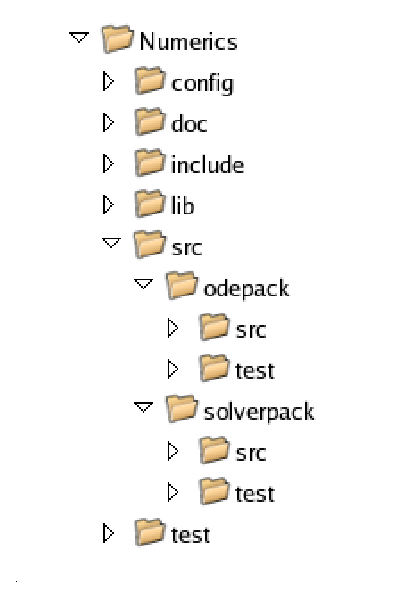
\includegraphics[scale=1.2, clip]{figure/NumericsDesign.eps}
	\caption{Tree view of the Numerics directories}
	\label{fig: Tree view of the Numerics directories}
	\end{center}
	\end{figure}




\begin{ndr}
put everywhere the main methods of the different modules\\
=> listing of the methods\\
\\
even if it's not very nice, it's a way to show the main methods that we can use
\end{ndr}


\section{Detailed design}
\subsection{\acs{lapack}}
%\begin{ndr}
%put here the funcitons used from LAPACK
%\end{ndr}
See the website dedicated to \ac{lapack} 
\begin{verbatim}( http://www.netlib.org/lapack/ ).\end{verbatim}
More details on the content of \ac{lapack} are available in this page 
\begin{verbatim}( http://www.netlib.org/lapack/lug/node19.html ).\end{verbatim}


\subsection{MP solverpack}
c.f. \ac{numerics} source code documentation generated by DOxygen.
\begin{ndr}
put here the information of the "poster" of solverpack
\end{ndr}


\subsection{\ac{ode} pack}
The functionalities given by \ac{ode} pack with \ac{numerics} are described in the documentation generated by DOxygen.
It correspond to the section called ...
\begin{ndr}
put the name of the .h of the C interface for ODE pack
\end{ndr}


%---------------------------------------------------------------------%

\newpage
\printglosstex(acr)[p]

%===================================

\listoffigures
\listoftables
\cleardoublepage
%\bibliographystyle{plainnat}
%\bibliography{./Biblio/String,./Biblio/Cp.bib,./Biblio/Optim.bib,./Biblio/Contact.bib,./Biblio/NonSmooth.bib,./Biblio/Leger.bib,./Biblio/Petri.bib}
\cleardoublepage
\end{document}
